\documentclass{homework}
\usepackage[utf8]{inputenc}
\usepackage{xspace,color,url,listings,graphicx,float,amsmath,amssymb,braket,subcaption}
\graphicspath{{./graphs/}} %location of images

\lstset{commentstyle=\color{red},keywordstyle=\color{black},
showstringspaces=false}
\lstnewenvironment{rc}[1][]{\lstset{language=R}}{}
\newcommand{\ri}[1]{\lstinline{#1}}  %% Short for 'R inline'

\lstset{language=R}             % Set R to default language

\newcommand{\hwname}{Shara Duong, Charles Colgan, Josh Borders}
\newcommand{\hwnum}{3}

\newcommand{\hwtype}{Homework}
\newcommand{\hwclass}{MATH 6350}

\begin{document}

\maketitle
Shara Duong: Wrote and edited code \\
Charles Colgan: Editeded text and code, created tables and figures\\
Josh Borders: Wrote and edited text, generated tables. \\

\textbf{Remark}: We replaced the font "Vladimir" with "Consolas," as the latter has substantially more complete cases, allowing us to better balanced the class sizes.

\question*{Correlation Matrix}
After centering and re-scaling the features by their means and standard deviations, respectively, we computed the correlation matrix of features (subset given in table \ref{tab:CORR}, full 400x400 correlation matrix in attached csv file). It demonstrates that neighboring features are highly correlated with one another. For example, pixels r0c1 and r0c2 have a correlation coefficient of 0.899. This is consistent with image data writ large. 
\begin{table}[h]
    \centering
    \begin{tabular}{c|cccccc}
      &r0c0&r0c1&r0c2&r0c3&r0c4\\
      \hline
r0c0&1.000&70.885&0.737&0.559&0.316\\
r0c1&0.885&1.000&0.899&0.703&0.432\\
r0c2&0.737&0.899&1.000&0.862&0.571\\
r0c3&0.559&0.703&0.862&1.000&0.801\\
r0c4&0.316&0.432&0.571&0.801&1.000
    \end{tabular}
    \caption{Correlation Matrix}
    \label{tab:CORR}
\end{table}
\\Our goal is to reduce the number of features required to still predict which font class a given case corresponds to, while maintaining a high degree of accuracy.

\question*{Eigenvalues and Eigenvectors}
We computed the eigenvalues and corresponding eigenvectors of the correlation matrix, the latter of which are stored in a matrix (5X5 subset in Table \ref{tab:EIG}, full 400x400 matrix in attached file).
\begin{table}[h]
    \centering
    \begin{tabular}{cccccc}
  e1&e2&e3&e4&e5\\
  \hline
  0.010&-0.014&0.068&-0.115&-0.033\\
  0.012&-0.004&0.072&-0.120&-0.030\\
  0.007&0.001&0.075&-0.127&-0.024\\
 -0.003&0.009&0.066&-0.124&-0.008\\
 -0.011&0.023&0.035&-0.103&0.016
    \end{tabular}
    \caption{Eignvectors}
    \label{tab:EIG}
\end{table}
\\Figure \ref{fig:EIG} displays a plot of the eigenvalues versus their count, r, of which there were 400. It demonstrates a strong, decreasing relationship, as the magnitude of the eigenvalues approach 0 around r=100. This indicates that we can reduce the dimension of the data from its current size to approximately 100, without losing much model performance.
\begin{figure}[h]
    \centering
    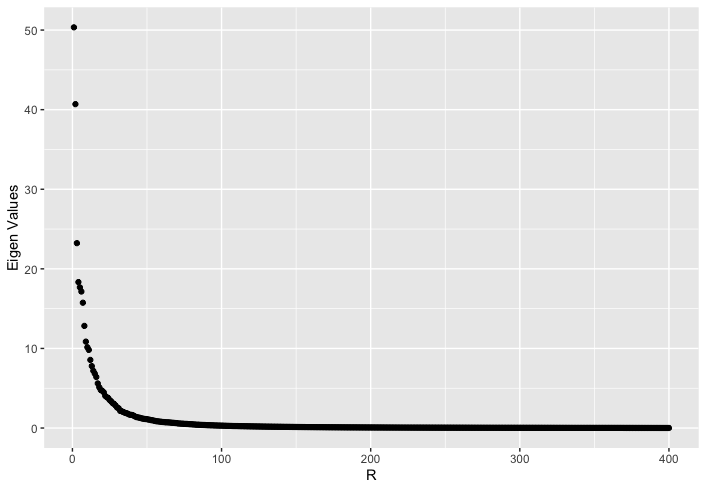
\includegraphics[width=8cm,height=6cm]{graphs/EIGEN.png}
    \caption{Eigenvalues vs. R}
    \label{fig:EIG}
\end{figure}

\question*{PVE and Principal Components}
Figure \ref{fig:PVE} plots the Proportion of Variance Explained vs R. An \textbf{r equal to 104 explains 95\% of the variance.}
\begin{figure}[h]
    \centering
    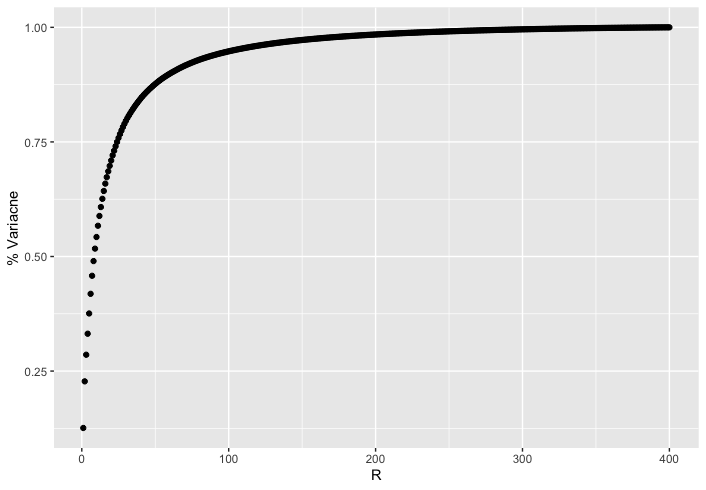
\includegraphics[width=8cm,height=6cm]{graphs/PVE.png}
    \caption{Proportion Variance Explained vs. R}
    \label{fig:PVE}
\end{figure}
\\We then computed the principal components by multiplying the original features by the transpose of the eigenvector matrix. 

\question*{New KNN}
We now run KNN using k=1 with the first 104 principal components. Table \ref{tab:CON} gives the confusion matrices for both training and testing sets. The classifier using PCA has a global accuracy on the training set of 99.5\%, while its global accuracy on the testing set is 85.1\%.\\ Without using the principal components, our KNN classifier at k=1 had a global accuracy on the training set of 99.6\%, and a global accuracy on the testing set of 84.6\%. The principal components boosted performance on the testing set by 0.5 percentage points.

\begin{table}[h]
    \centering
    \subfloat[train]{\begin{tabular}{c|ccc}
         &BITSTREAM&CONSOLAS&EBRIMA\\\hline
         BITSTREAM&1.00&0.00&0.00\\
         CONSOLAS&0.00&1.00&0.00\\
         EBRIMA&0.00&0.02&0.98
    \end{tabular}}\\
    \subfloat[test]{\begin{tabular}{c|ccc}
         &BITSTREAM&CONSOLAS&EBRIMA\\\hline
         BITSTREAM&0.97&0.02&0.01\\
         CONSOLAS&0.04&0.83&0.13\\
         EBRIMA&0.06&0.22&0.72
    \end{tabular}}
    \caption{Confusion Matrix. True class is by row, Predicted class is by column}
    \label{tab:CON}
\end{table}

\question*{Plots}
Figure \ref{fig:SCA} displays scatter plots in the plane for the first six pairs of the principal components Y$_1$, Y$_2$, Y$_3$, Y$_4$. Each font is represented by a colored point: red for Bitstream, green for Consolas, and blue for Ebrima. Plotting the first few pairs does not yield clear separation between the font classes. This is ultimately not that surprising, as it required 104 principal components (i.e., 104 dimensions) to explain 95\% of the variance in the data. These two-dimensional scatter plots, while aesthetically pleasing, do not provide insight that one principal component is substantially better at predicting font class than any other.
\pagebreak
\begin{figure}[h]
    \centering
    \subfloat[]{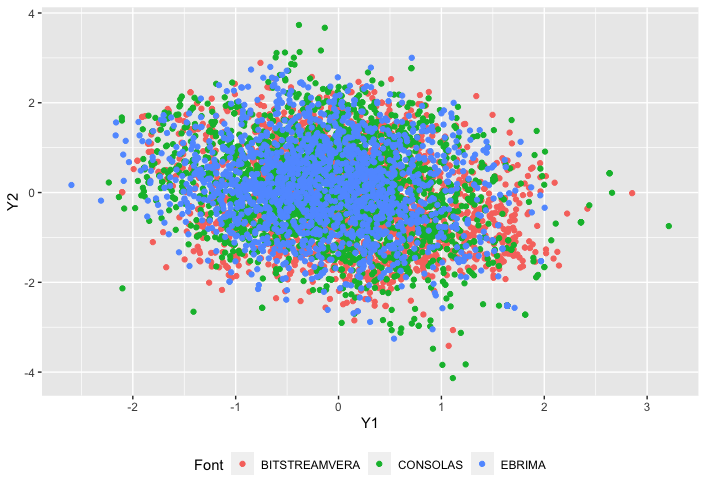
\includegraphics[width=7cm,height=4.5cm]{graphs/SCA1,2.png}}
    \subfloat[]{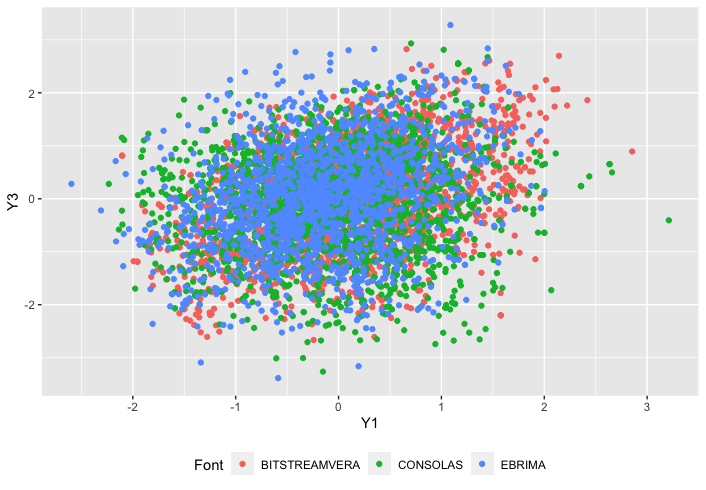
\includegraphics[width=7cm,height=4.5cm]{graphs/SCA1,3.png}}\\
    \subfloat[]{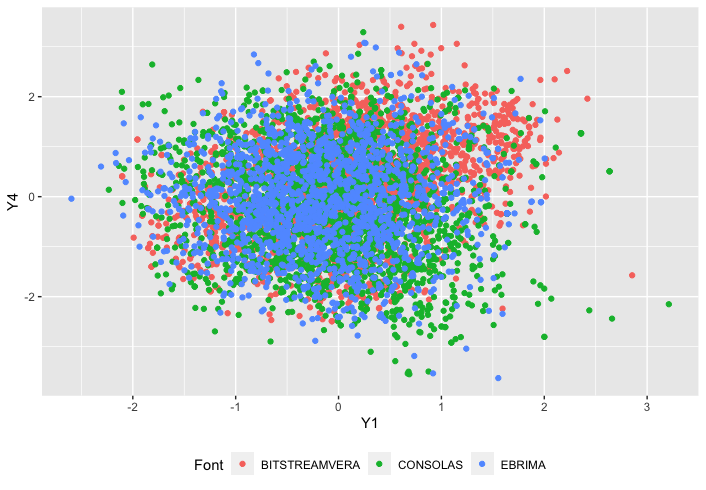
\includegraphics[width=7cm,height=4.5cm]{graphs/SCA1,4.png}}
    \subfloat[]{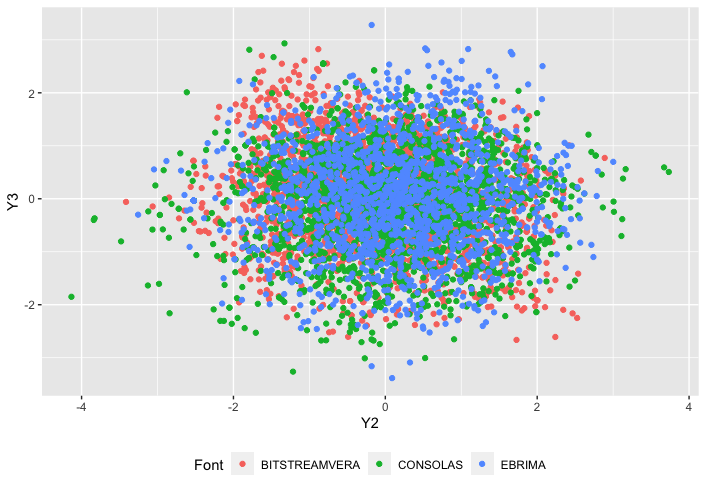
\includegraphics[width=7cm,height=4.5cm]{graphs/SCA2,3.png}}\\
    \subfloat[]{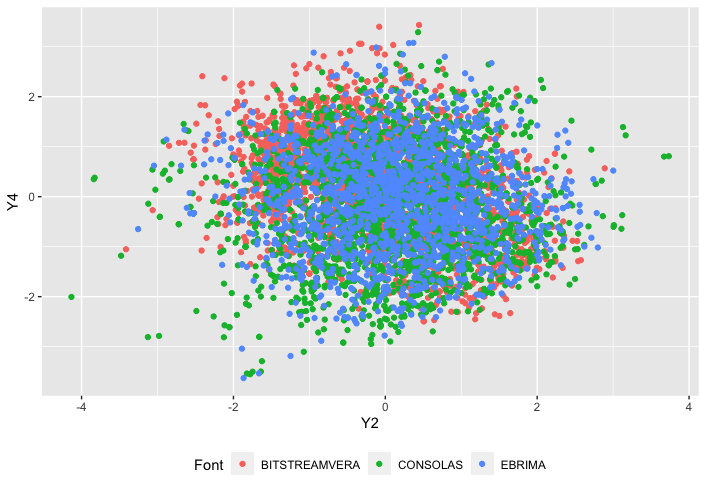
\includegraphics[width=7cm,height=4.5cm]{graphs/SCA2,4.png}}
    \subfloat[]{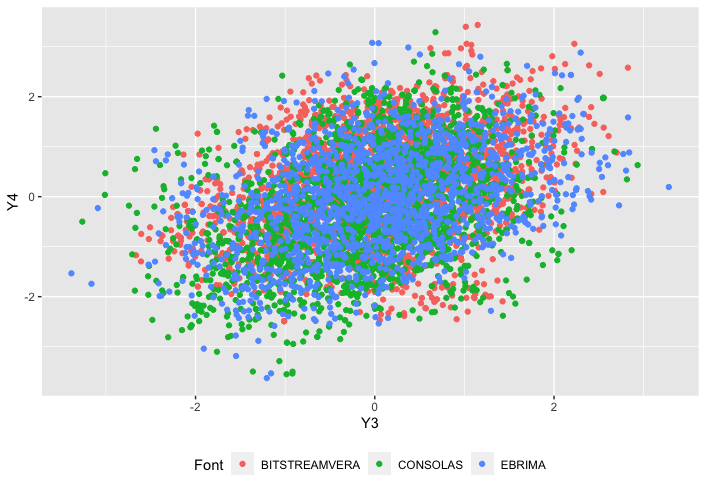
\includegraphics[width=7cm,height=4.5cm]{graphs/SCA3,4.png}}
    \caption{Scatter Plots for First Four Principal Components}
    \label{fig:SCA}
\end{figure}
\newpage
\lstinputlisting{code.R}
\end{document}
